\chapter{Buggy Construction and Performance Requirements}

	Each buggy shall have been designed and constructed by eligible undergraduate or graduate students of Carnegie Mellon University. These students shall also have been members of the buggy's sponsoring organization at the time that they designed and constructed the buggy. Last semester seniors shall be considered
	to be full-time students.

	Buggies may be borrowed/loaned or bought/sold by one organization from or to another organization, provided that the Sweepstakes Chairman is notified of the Transition, and it takes place before heats and lanes are selected for the preliminary races (if that buggy is to be used in those races). Provided the buggy passes construction, safety, and performance requirements, it will be eligible to roll for the new organization. If needed, an alumni that owns an eligible buggy may provide it to be loaned/sold provided it satisfies the Buggy Construction and Performance Requirements, undergoes a rigorous safety inspection by the Sweepstakes Safety Chair, and passes the braking capability and drop brake tests.

\section{Braking System}

	Each buggy shall have a driver operated system or mechanism which is capable of stopping the rolling motion
	of that buggy. This system or mechanism shall be known as the buggy's braking system. Each buggy's
	braking system shall be capable of passing two separate braking performance tests, the braking capability
	test and the drop brake test. In addition, all braking systems must meet the following requirements:


	\begin{itemize}

		\item
		The brakes shall be self-resetting. This means that the brakes shall release their braking force whenever
		the driver stops actuating them.


		\item
		The brakes shall be capable of being actuated to full braking force, and then be completely released,
		at least three times in succession, without any maintenance.
		

		\item
		All fasteners and hardware used in the braking system shall be equipped with locking devices, such as
		lock nuts, lock washers, lock wires, cotter pins, etc. The use of anaerobic locking compounds (such as
		Loctite) is permissible, but is not sufficient. Tubing fittings used in hydraulic or pneumatic braking
		systems need not be equipped with locking devices, with the approval of the Safety Chairman, due to
		the inherent vibration resistance of these fittings alone.
		

	\end{itemize}

\subsection{Braking Capability Test}

	Each buggy shall pass a braking capability test, at least once each school semester, with each person who will be driving it, before that person will be permitted to drive that buggy in any type of practice session at
	Carnegie Mellon University during that semester. 
	
	The purpose of the braking capability test is to ensure that each buggy meets a minimum breaking standard when moving in the forward direction, while a particular person is driving it.  The braking capability test shall be administered by the Safety Chairman, or anyone designated by that Chairman.

	The test shall take place on a flat, level, and smooth area, that is paved with either concrete or asphalt.If the area chosen is not completely level, the test shall be run in a direction such that the buggy being tested shall be moving toward the lower end of the area during the test. The sidewalk starting at Purnell and moving towards the University Center shall be used if it is available and in acceptable condition. If this area is not available or acceptable the Safety Chairman, or anyone designated by that Chairman, shall choose an alternate location for the test. A buggy may be tested for rearward braking at any time by the safety chairman as part of a spot safety check.


	\begin{center}
		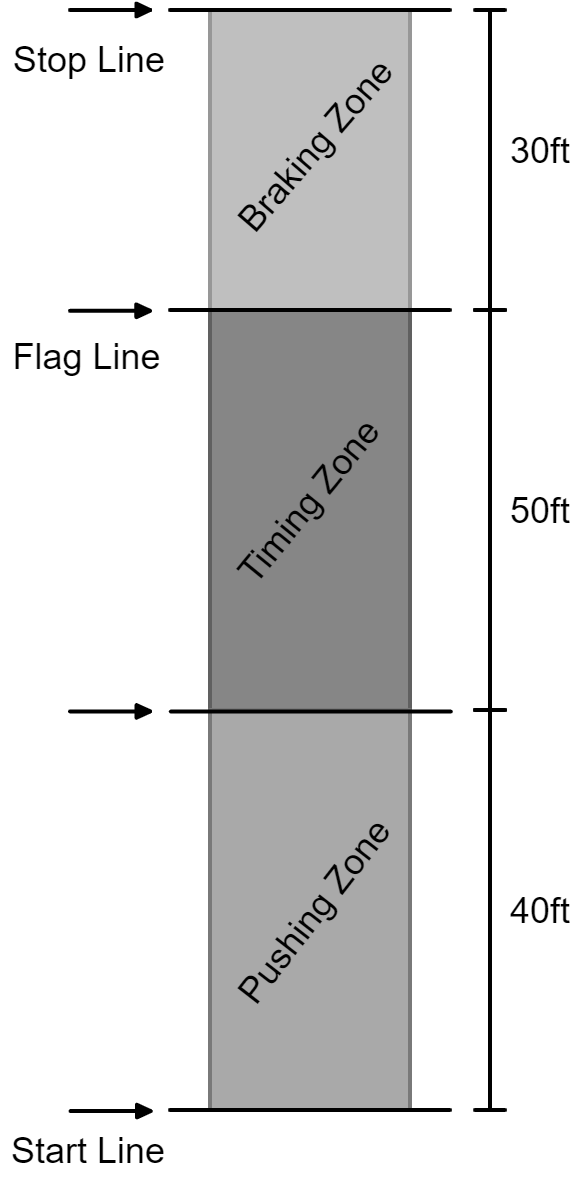
\includegraphics[height=4in]{assets/Buggy-Brake-Test-gs.png}
	\end{center}
	
	The test shall be conducted as follows:

	\begin{itemize}

		\item
		The buggy shall be pushed through a 40 ft long pushing zone such that it is moving at a speed greater than or equal to 15 miles per hour (22 feet per second).


		\item
		After the pusher releases the buggy, the average speed of the buggy shall be measured while the buggy travels through a 50 foot long timing zone. The average speed of the buggy shall be determined by measuring the time required for the nose of the buggy to travel from the beginning to the end of the 50 foot long timing zone. A stopwatch or other suitable timing device shall be used to make this measurement.

		\item
		When the nose of the buggy reaches the end of the 50 foot long timing zone, the driver shall be signaled to apply the buggy's brakes.

		\item
		After the buggy stops, the test administrator shall tell the driver to release and reapply the brakes two more times, while the administrator is pushing on the buggy's pushbar to verify that the brakes are being released and reapplied.

		\item
		Two members of the buggy's sponsoring organization shall be located in a position such that they will be able to stop the buggy in the event that the buggy's braking system fails to stop the buggy during the test.

		\item
		The organization whose buggy is being tested shall provide an adequate number of people to control pedestrian traffic in the test area and to properly attend to all of the buggies that they are using. If the braking capability test is performed between sunset and sunrise, any buggy that is tested must have all lights and reflectors that are required during night push practices.


	\end{itemize}

	To successfully complete the test, the following requirements must be met:

	\begin{itemize}

		\item
		Only the driver may touch the buggy while it is being tested.

		\item
		The average speed of the buggy while it is traveling through the 50 foot long timing zone must be determined to be 15 miles per hour (22 feet per second) or greater.


		\item
		The buggy must stop within the distance prescribed by the schedule that follows. This schedule lists the measured time required for the buggy to travel through the 50 foot long timing zone and the average speed of the buggy through that zone. The buggy must then stop within 30 ft (measured to the nose).


			\begin{tabular}{c c c}
				Measured Time & Average Speed  \\
				2.25 sec. & 15.2 mph (22.2 fps)\\
				2.20 sec. & 15.5 mph (22.7 fps)\\
				2.15 sec. & 15.9 mph (23.3 fps)\\
				2.10 sec. & 16.2 mph (23.8 fps)\\
				2.05 sec. & 16.6 mph (24.4 fps)\\
				2.00 sec. & 17.0 mph (25.0 fps)\\
				1.95 sec. & 17.5 mph (25.6 fps)\\
				1.90 sec. & 17.9 mph (26.3 fps)\\
				1.85 sec. & 18.4 mph (27.0 fps)\\
				1.80 sec. & 18.9 mph (27.8 fps)\\
				1.75 sec. & 19.5 mph (28.6 fps)\\
				1.70 sec. & 20.1 mph (29.4 fps)\\
			\end{tabular}

		\item
		While the buggy is stopping, its centerline must not deviate more than 15 degrees from the line that it was moving along, in the 50 foot long timing zone.


		\item
		After the buggy has stopped, it must remain in a stable position with no external assistance, and its driver must successfully release and reapply its brakes two additional times.


		\item
		The buggy's brakes may not be applied during the 50 foot long timing zone

	\end{itemize}

	If a buggy fails to successfully complete the braking capability test during any four consecutive attempts on any one day, that buggy shall not be permitted to attempt the braking capability test again for a period
	of 24 hours. Attempts where the buggy travels through the timing zone in fewer than 2.1 sec (~24 fps) and does not stop within 30 ft shall not count toward an attempt and the team shall be instructed to try again at a slower speed. Performing the test outside of the speed requirements cannot be used to break up consecutively failed brakes tests. 
	
	The buggy shall be in the same physical state as would be expected for regular free rolls practice. No tactics may be employed to aid in passing the drop test or slowing forward motion of the buggy that would not be used in an emergency condition on the course. Actions not allowed include but are not limited to: overtightening of the retaining mechanism on wheels, use of spacers or shims to cause additional friction, use of worn or dirty bearings, and objects dragging on the ground. Any organization's buggy caught violating this policy will be treated as if it failed a spot safety check.

\subsection{Drop Brake Test}

Each buggy is required to take a drop brake test with each person who will be driving it that day before every freeroll practice, after it competes in any race, and whenever the Sweepstakes Chairman, the Assistant Sweepstakes Chairman, or the Safety Chairman request such a test. The purpose of the drop brake test is to demonstrate that the buggy's brakes are in proper working order and that the driver is able to actuate them. The drop brake test shall be administered by the Sweepstakes Chairman, Assistant Sweepstakes Chairman, Safety Chairman,or anyone designated by any of these Chairmen.

The procedure for the drop brake test shall be as follows:

The test shall take place somewhere on one of the sidewalks of Tech Street, along Hill 1 of the buggy course. The sidewalk directly in front of the middle entrance to Skibo Gymnasium shall be used if it is available and is in acceptable condition. If this area is not available or acceptable, the Safety Chairman, or
anyone designated by that Chairman, shall choose an alternate location for the test.

The test shall be conducted as follows:
\begin{itemize}
	\item The buggy shall be placed at rest on the sidewalk facing toward the bottom of the hill, with its nose at the beginning of a marked 30 foot long zone.

	\item The buggy shall be released and allowed to roll down the hill without being inhibited, to the bottom end of the 30 foot long zone.
 
	\item When the buggy reaches the end of the 30 foot long zone, the driver shall be signaled to apply the buggy's brakes.
 
	\item After the buggy stops, the test administrator shall tell the driver to release and reapply the brakes once, while observing the movement of the buggy to verify that the brakes are being released and reapplied.
 
	\item A member of the buggy's sponsoring organization shall be located in a position such that they will be able to stop the buggy in the event that the buggy's braking system fails to stop the buggy during the test.
 
	\item The organization whose buggy is being tested shall provide an adequate number of people to control pedestrian traffic in the test area and to properly attend to all of the buggies that they are using. If the drop brake test is performed between sunset and sunrise, any buggy that is tested must have all lights and reflectors that are required during night push practices.
\end{itemize}

To successfully complete the test, the following requirements must be met:
\begin{itemize}
	\item Only the driver may touch the buggy while it is being tested.
 
	\item The buggy must stop within 15 feet of the end of the 30 foot long zone through which it has been allowed to roll. This 15 foot distance shall be measured to the nose of the buggy, i.e. that part of the buggy that is farthest away from the end of the 30 foot long zone.
 
	\item After the buggy has stopped, its driver must successfully release and reapply its brakes once.
 
	\item The buggy's brakes must not be applied before the buggy reaches the end of the 30 foot long zone through which it has been allowed to roll.
\end{itemize}

The buggy shall be in the same physical state as would be expected for regular free rolls practice. No tactics may be employed to aid in passing the drop test or slowing forward motion of the buggy that would not be used in an emergency condition on the course. Actions not allowed include but are not limited to: overtightening of the retaining mechanism on wheels, use of spacers or shims to cause additional friction, use of worn or dirty bearings, and objects dragging on the ground. Any organization's buggy caught violating this policy will be treated as if it failed a spot safety check.


\section{Configuration}

	There shall be no restrictions on the configuration that a buggy may have with respect to the position of the driver, the type of braking system, the location of the braking system, the type of steering system, and the type of frame, as long as the buggy complies with all of the design, construction, and performance criteria specified in these Rules, Regulations, and Procedures.

\section{Driver's Personal Protection}

	All new helmets and harnesses must be tagged by Sweepstakes at their first use and teams must provide a receipt with date of purchase. Helmets and harnesses must be retired after 5 years of their first use. These tags will clearly indicate when that piece of equipment must be taken out of circulation and replaced. Additionally, Sweepstakes will maintain a running log of safety equipment. 

\subsection{Eye Protection}

	Drivers MUST wear approved goggles with anti fogging compounds or solutions applied whenever they are driving a buggy. The goggles must have shatterproof lenses, and must provide side-shield protection to the eyes. Any goggles that are examined by the Safety Chairman and are deemed to be adequate, or that meet the requirements of ANSI Z87.1, are considered to be approved goggles. Goggles with clear or tinted lenses may be used by buggy drivers when they are driving a buggy anytime after sunset and before sunrise. A driver with visual acuity of less than 20/40 combined vision SHALL wear lenses correcting combined vision to 20/40 or greater at all times while driving a buggy. These corrective lenses shall be in addition to or part of the goggles specified above.

\subsection{Hand Protection}

	Drivers MUST wear suitable gloves whenever they are driving a buggy. Gloves must help reduce the chances of cuts and abrasions in the event of an accident. The gloves should cover all parts of both hands, including the fingers, thumbs, palms, and the backs of the hands. All gloves must be approved by the Safety Chairman.

\subsection{Mouth Protection}

	Drivers MUST wear an approved mouthguard whenever they are driving a buggy. Approved mouthguards meet the ANSI/ADA Specification 99-2001 and must protect at least the upper jaw as well as provide some type of custom fitting, such as boil and bite or custom fitted mouthguards. Difficulty speaking or breathing generally indicates an incorrectly fitted mouthguard. Stock mouthguards provide inadequate protection and are NOT approved for use.

\subsection{Head Protection}

	Drivers MUST wear an approved hard shell helmet whenever they are driving a buggy. The follow styles of helmet are approved for use: 
	\begin{itemize}
		\item A rock climbing helmet with the CE-EN 12492 and UIAA rating
		\item A bicycle helmet with at minimum the CPSC rating, although a SNELL rating is preferred 
		\item A hockey helmet with a CSA rating (CAN3-Z262.2-M78 or Z262.1) 
	\end{itemize}

	The helmet must not restrict the movement of the driver or the driver's head while the buggy is being driven. Helmets should be replaced every five years, or in accordance with crash replacement guidance per Safety Chairman and EH\&S. Rock climbing helmets are preferred over other types of helmet. 
	
	Helmets MUST be fitted to each driver according to the manufacturer's guidelines, excepting the modifications detailed below. They should not move out of place or obstruct the driver's vision at any time, even under the application of significant force.

\subsubsection{Modifications}

	Helmets may not be modified by cutting, removing or altering the lining, padding, shell, or chin strap in any way except as follows:
	\newline

	The shell, lining, and padding of the helmet may be trimmed away in the upper front area of the helmet (above where the driver's forehead would be) in order to provide adequate vision for the driver. The section trimmed away shall be in the shape of a smooth arc no more than 1.5 inches high (at its greatest height) by 5.0 inches wide (at its widest point.) The edges of the trimmed away section of the helmet shall be smoothed, beveled, and/or padded in order to reduce the possibility of injury to the driver while the helmet is being worn. In no case may any stiffening ribs or supporting members of the helmet shell be removed or altered in any way. Any modifications made to a helmet must be approved by the Safety Chairman before the modified helmet can be used by a buggy driver.
	
	A helmet may also be modified, as described above, in the lower rear area (where the back of the driver's neck would be) in order to provide adequate head tilt for the driver. The requirements are the same as described above except that the maximum dimensions of the cut away area shall be 2.0 inches high by 5.0 inches wide.

	Any team modifying their helmets must disclose so during capabilities testing with the Safety Chair. Buggies which finish construction after the 2023-2024 school year must NOT use modified helmets.

\subsection{Safety Harness}

	Drivers MUST wear an approved safety harness whenever they are driving a buggy. Any harness that is examined and deemed to be acceptable by the Safety Chairman, or is supplied through the Sweepstakes Advisor, is considered to be an approved harness. 

	Each buggy shall pass a pull capability test, at least once each school semester, with each person who will be driving it, before that person will be permitted to drive that buggy in any type of practice session at Carnegie Mellon University during that semester. 

	The purpose of the pull capability test is to physically demonstrate the security of the harness and attachment points. The pull capability test shall be administered by the Safety Chairman, or anyone designated by that Chairman. The test shall take place at the same location as the braking capability test. 

	The test shall be conducted as follows: 
	\begin{itemize}
		\item
		The buggy will be supported in order to raise its wheels off the ground or firmly held in place to prevent it from moving

		\item
		The driver will be fully loaded into the buggy
	
		\item
		The tester will take the driver's hands and pull		
	\end{itemize}

	In order to pass this test, drivers must not be displaced more than an inch after being pulled. 


\subsubsection{Attachment}

	Every driver's safety harness must be attached to that driver's buggy at a minimum of three different points, whenever that person is driving that buggy. These attachments shall only be made to structural members of the buggy, and they shall be such that the movement of the driver is restricted in all directions (i.e. forward, rearward, side to side, and vertical)such that in the event of an impact to the buggy from any direction, the driver shall be retained inside, but not impact against, the driver's protective cage. All harness attachment points shall be approved by the Safety Chairman during the buggy's safety inspection.
	
	Safety harnesses must have the capability to permit quick and easy removal of the driver from the buggy in the event of an accident or other problem while the driver is secured in the buggy with the safety harness. This removal must be possible without the use of tools or other mechanical devices.

\subsubsection{Construction}

	The straps from which a safety harness is constructed must be at least 1.75 inches wide. This is to ensure that the forces of a collision are distributed over a relatively large area of a driver's body. Standard automotive seat belt material is acceptable. With the approval of the Safety Chairman, the lower portion of a safety harness may consist of a commercially available rock climbing harness, even though its straps may be less than 1.75 inches wide.

\subsubsection{Additional Safety Harness Requirements}

	All harness clips must be d-ring carabineers and certified by the UIAA (International Mountaineering and Climbing Federation).
	
	All box stitching on the harness must be completed by professional stitchers, performed on a heavy duty industrial sewing machine, and deemed adequate by the Safety Chairman. In the event that the Safety Chairman does not believe the stitching was professionally done, the buggy organization's Chairman must show a receipt indicating that a professional performed the stitching. In the event that the Chairman does not have the receipt the harness will be deemed unsafe and will not pass the safety. 
	
	Harnesses can be bought from stores, provided that they comply with the rules listed in this section. Many rock climbing stores sell harnesses that comply to the rules.

	When attaching a driver's harness to a buggy, no part of the harness or attachment method may be made up of a fabric, rope, or textile, which has been pierced through. Exceptions may be made for professional stitching like that described for harnesses.

\section{Driver's Protective Cage}

	Each buggy shall be constructed with a structurally sound cage which totally surrounds the driver. The purpose of this cage is to help protect the driver from front, side, rear, and rollover impacts in the event of an accident. The driver's protective cage shall meet the following minimum requirements:

	NO PART of the driver's body shall extend beyond the protective cage.
	The interior of the protective cage shall not have any sharp edges, pointed objects, or protruding objects, which could injure the driver in the event that the driver is pushed into or thrown against these edges or objects.
	None of the wheels of the buggy shall be considered to be part of the driver's protective cage.
	The protective cage shall be designed and constructed in such a way that injury to the driver will be minimized in the event that one or more of the buggy's wheels become detached from the buggy, while it is moving.
	The protective cage shall be designed and constructed in such a way that a 1.0 inch wide by 72 inch long infinitely stiff bar, held in ANY position in a vertical plane perpendicular to the centerline of the buggy (this means with the bar's axis vertical, horizontal, or at any angle,) will not intrude into the front of the cage, nor contact any part of the driver's body, nor increase the force distribution on the driver's body, when pushed toward the buggy with a force of 1,000 pounds, while the buggy is restrained so that it cannot move.

	The protective cage shall be designed and constructed in such a way that a 2.0 inch wide by 12 inch long infinitely stiff bar, held in ANY position (see preceding paragraph) in any vertical plane that is either perpendicular to or parallel to the centerline of the buggy, will not intrude into the sides or rear of the cage, nor contact any part of the driver's body, nor increase the force distribution on the driver's body, when pushed toward the buggy with a force of 500 pounds, while the buggy is restrained so that it cannot move.
	The protective cage shall be designed and constructed in such a way that it shall not collapse or deform such that any part of the driver's body would be contacted (by the cage or by the steel plate,) if a 2 ft. by 5 ft. by 1.00 inch thick steel plate was slowly lowered onto the top of the buggy. (This plate weighs approximately 408 pounds.)
	If a buggy has a pushbar that can change its position (this means that it is not rigidly and permanently attached to the buggy,) that pushbar shall NOT be considered to be a part of that buggy's protective cage.
	Any buggy with such a pushbar, must meet all of the requirements for the driver's protective cage with its pushbar in any of its possible positions. This is to ensure that the pushbar itself, will not cause an injury to the driver in the event of an accident.
	The protective cage shall be designed and constructed in such a way that no part of the driver's body shall be exposed to the road surface. The purpose of this requirement is to ensure that there is some substantial structure protecting the driver from below in the event that the bottom of the buggy comes in contact with another object, such as if the wheels came off and the buggy slid along the ground.

	Each buggy shall pass a structural capability test, at least once each school semester, with each person who will be driving it, before that person will be permitted to drive that buggy in any type of practice session at Carnegie Mellon University during that semester. 

	The purpose of the structural capability test is to physically demonstrate the safety of the shell by applying a distributed load to it. The structural capability test shall be administered by the Safety Chairman, or anyone designated by that Chairman. The test shall take place at the same location as the braking capability test. 

	The test shall be conducted as follows: 
	The buggy will be placed on the ground, or supported for each axle of the buggy 
	One or more individuals will sit on the buggy such that a load of approximately 150 lbs (minimum) is applied to the shell of the buggy. (No more than 400 lbs will be required for the test)
	The tester will then apply pressure to the outside of the buggy to check for delamination along the shell

	To pass this test, the buggy must not sustain structural damage after being sat on and the buggy must not show signs of extensive delamination. The metric for extensive delamination is left to the judgment of the Safety Chair or anyone appointed by the Safety Chair.

\section{Field of Vision}

	Each buggy shall pass a field of vision test, at least once each school semester, with each person who will be driving it, before that person will be permitted to drive that buggy in any type of practice session at Carnegie Mellon University during that semester. The purpose of the field of vision test is to ensure that each buggy provides a minimum field of vision to each person who will be driving it. The field of vision test shall be administered by the Safety Chairman, or anyone designated by that Chairman. The test shall take place at the same location as the braking capability test.
	The test shall be conducted as follows:

	\begin{itemize}

		\item
		The driver to be tested shall be placed inside the buggy with all of the driver's personal protection equipment in place as it would be if the driver were going to drive the buggy, i.e. wearing a properly secured helmet, a safety harness, goggles, and gloves.

		\item
		The buggy shall be aligned in such a way that a 90 degree angle, whose origin is located at the point where the centerline of the buggy and the buggy's front axle intersect, and whose bisector is coincident with the centerline of the buggy, can be determined.

		\item
		The tester may hold up between 0 and 10 fingers throughout the 90 degree range. The driver inside the buggy shall be asked if they can identify how many fingers the tester is holding up, and features and objects on the horizon beyond.

	\end{itemize}

	To successfully complete the test, a driver inside the buggy must have a viewing range enabling them to to identify features and objects on the horizon at any angle less than 45 degrees from the centerline in the direction of straight travel. The driver must also identify the number of fingers the tester is holding up anywhere within this viewing range, at ground level 25 feet from the front axle.

\section{Pushbar}

	Each buggy shall have a structure which its pushers can push on, in order to propel that buggy forward. This structure shall be known as a pushbar. Each pushbar shall have a structurally sound cross-piece at its end, which shall be known as the pushbar handle. The pushbar handle will usually be perpendicular to the pushbar and, to ensure safety, should have the recommended, but not required, dimensions of 8 inches long by 1 inch in diameter.

	If any part of a buggy's pushbar moves from the position that it is normally in when its pushers are propelling that buggy forward, that part or parts of that pushbar may only move to a position that is inside the driver's protective cage, or to a position that is directly above the outline of the driver's protective cage when viewed from above the buggy. During any such movement, no part of the pushbar may extend below or behind the normal pushing position of the pushbar unless it is also within or above the outline of the driver's protective cage at the same time.

\section{Buggy Restrictions}

	\begin{itemize}

		\item
		No buggy may have any device whose purpose is to store energy independent of the speed of the buggy (such as a geared flywheel) or whose purpose is to increase the forward speed of that buggy by adding kinetic energy to that buggy.

		\item
		No buggy may have any means of internal propulsion.

		\item
		Exceptions are made for robotic buggies to store energy and use internal propulsion in order to operate their systems; however this energy must not increase the forward speed of the buggy. 

		\item
		No buggy may have any type of protrusion (such as a sharp and/or pointed structure) extending from that buggy which could increase the likelihood of injury to the driver of another buggy in the event of an accident. The nose/tail of a buggy should be parabolic and not come to a point. If it were a curve, the derivative of any point on that curve should be defined across the whole length. This prohibits nose and tails that come to a point in three or two dimensions (i.e. a true point or an edge.) An allowed exception to this would be flat or cut-off tails, though the flat face must form an angle between 45 and 90 degrees to the ground. The minimum radius of curvature permitted for any nose or tail is .75. Final discretion as to what might be considered overly pointy is up to the discretion of the Safety Chairman.

		\item
		No buggy may be designed such that it would intentionally have less than three wheels in contact with the ground whenever it is on the buggy course.

	\end{itemize}

\section{Shell}

	Each buggy shall have a means to securely attach its shell, hatch, or cover, if that part of the buggy is removable. The use of magnetic attachments is permissible but it is not sufficient, adequate attachments include but are not limited to pins, screws, and bolts. The adequacy of any attachment shall be determined by the Safety Chairmen, during the buggy’s safety inspection.


\section{Size}

	A 15' long by 6' wide rectangle including the pushbar is the maximum footprint of a buggy. Width is defined as perpendicular to the direction of straight travel.

\section{Steering System}

	Each buggy shall have a driver operated system or mechanism that shall control and determine the direction in which that buggy will move, whenever that buggy is in motion. This system or mechanism shall be known as that buggy's steering system. Each buggy's steering system shall:

	\begin{itemize}

		\item
		Be Designed such that the driver will be able to control the buggy under all normal driving conditions.

		\item
		Operate in a smooth and stable manner. The steering system shall not bind or behave in an erratic way during use, such that it might cause the driver to lose control of the buggy. The steering mechanism should also usually tend to return to a neutral (straight ahead) position when no steering inputs are received from the driver.

		\item
		Equip all fasteners and hardware with locking devices. Fasteners and hardware include nuts, bolts, collars, etc., used to attach or secure any part of a buggy's steering system. Acceptable locking devices include lock nuts, lock washers, lock wires, cotter pins, etc. The use of anaerobic locking compounds (such as Loctite) is permissible, but is not sufficient.

	\end{itemize}

Each buggy shall pass a steering capability test, at least once each school semester, with each person who will be driving it, before that person will be permitted to drive that buggy in any type of practice session at Carnegie Mellon University during that semester. 

The purpose of the steering capability test is to ensure each driver is able to properly steer each buggy they will be driving both left and right with sufficient responsiveness. The steering capability test shall be administered by the Safety Chairman, or anyone designated by that Chairman. The test shall take place at the same location as the braking capability test. 

The test shall be conducted as follows: 
\begin{itemize}
	\item	
	The driver must be wearing all equipment needed to drive

	\item
	The buggy shall start in the center of the area normally used for brake testing
	
	\item
	The driver will be instructed to follow the feet of the tester

	\item
	The tester will walk a serpentine path while another individual slowly walks the buggy forward
\end{itemize}

The tester will then evaluate the turning capability of the buggy, ensuring that the driver is able to turn both left and right, and that they have a sufficient turning radius. Having sufficient steering is left to the judgment of the Safety Chair or anyone appointed by the Safety Chair. 


\section{Wheels}

	All fasteners and hardware (i.e. nuts, bolts, collars, etc.) that are used to secure a buggy's wheels to that buggy shall be equipped with locking devices such as lock nuts, lock washers, lock wires, cotter pins, etc. The use of anaerobic locking compounds (such as Loctite) is permissible,but is not sufficient.

	No buggy may use any official soap box derby race wheels if those wheels are constructed of any type of plastic material. Experience has shown that these wheels, while adequate for straight line soap box derby racing, are structurally deficient in buggy racing applications.

\section{Windscreens}

	Each buggy shall have a windscreen with anti fogging compounds or solutions applied in front of the driver's face in order to help protect the driver from wind, dust, flying objects, and debris. Each windscreen shall be made of clear polycarbonate plastic, also trademarked LEXAN (R) General Electric. The minimum nominal thickness for each windscreen shall be 0.062 inches.
	
	Each buggy's windscreen shall be mechanically attached to structural members of that buggy such that in the event of an impact to that windscreen, the windscreen will fail before the windscreen's supporting members will fail. Each windscreen shall be secured along more than two of its edges with mechanical fasteners (such as bolts, rivets, etc.) that are approved by the Safety Chairman. Attachment of the windscreen to the buggy with duct tape or other types of tape is permissible, but is not sufficient.
	
	The use of tinted or mirrored windshields on buggies during after dark practice sessions must be approved by the Safety Chairman.

\subsection{Interior Debris Shield}

	Any buggy which has a wheel located in front of the driver, shall also have a protective shield between that wheel and the driver's face. The purpose of this shield is to reduce the possibility of debris being thrown into the driver's eyes and/or face by the wheel. This debris could come from either the road surface or from the wheel itself in the event that the tire fails and breaks into pieces. This shield shall meet the requirements of one of the following options:

	\begin{itemize}

		\item
		This shield shall be durable, shatterproof, and conform to the shape of the wheel. To meet the minimum requirements, it shall cover the entire line-of-sight path between the driver's head and the nearest half of the wheel. This shield shall have both a diameter and width no more than 1 inch greater than the wheel itself, and a minimum nominal thickness of 0.031 inches may be used.

		\item
		This shield shall be made of clear polycarbonate plastic, which has a minimum nominal thickness of 0.062 inches, also trademarked LEXAN (R) General Electric. It shall extend from the bottom of the buggy to the top of the buggy, and shall be at least 4.0 inches wide.

	\end{itemize}

	Regardless of implementation, the shield shall be attached to a structural member of the buggy with mechanical fasteners (such as bolts, rivets, etc.) and its attachment method shall be approved by the Safety Chairman during the buggy's safety inspection.
